\documentclass{standalone}

\usepackage[T1]{fontenc}
\usepackage[utf8]{inputenc}
\usepackage{eulervm}
\usepackage{pgfplots}

\pgfplotsset{compat=newest}
\usepackage{color}

\definecolor{Comment}{RGB}{97,161,176}

\definecolor{btfGreen}{RGB}{51,160,44}
\definecolor{btfRed}{RGB}{190,60,90}

\definecolor{bleuUni}{RGB}{0, 157, 224}
\definecolor{marronUni}{RGB}{68, 58, 49}
\definecolor{grayMarronUni}{RGB}{60, 60, 60}
\definecolor{grayBleuUni}{RGB}{118, 118, 118}

\definecolor{bluecite}{HTML}{009DE0}

\definecolor{Paired-2}{RGB}{166,206,227}
\definecolor{Paired-1}{RGB}{31,120,180}
\definecolor{Paired-4}{RGB}{178,223,138}
\definecolor{Paired-3}{RGB}{51,160,44}
\definecolor{Paired-6}{RGB}{251,154,153}
\definecolor{Paired-5}{RGB}{227,26,28}
\definecolor{Paired-8}{RGB}{253,191,111}
\definecolor{Paired-7}{RGB}{255,127,0}
\definecolor{Paired-10}{RGB}{202,178,214}
\definecolor{Paired-9}{RGB}{106,61,154}
\definecolor{Paired-12}{RGB}{255,255,153}
\definecolor{Paired-11}{RGB}{177,89,40}
\definecolor{Accent-1}{RGB}{127,201,127}
\definecolor{Accent-2}{RGB}{190,174,212}
\definecolor{Accent-3}{RGB}{253,192,134}
\definecolor{Accent-4}{RGB}{255,255,153}
\definecolor{Accent-5}{RGB}{56,108,176}
\definecolor{Accent-6}{RGB}{240,2,127}
\definecolor{Accent-7}{RGB}{191,91,23}
\definecolor{Accent-8}{RGB}{102,102,102}
\definecolor{Spectral-1}{RGB}{158,1,66}
\definecolor{Spectral-2}{RGB}{213,62,79}
\definecolor{Spectral-3}{RGB}{244,109,67}
\definecolor{Spectral-4}{RGB}{253,174,97}
\definecolor{Spectral-5}{RGB}{254,224,139}
\definecolor{Spectral-6}{RGB}{255,255,191}
\definecolor{Spectral-7}{RGB}{230,245,152}
\definecolor{Spectral-8}{RGB}{171,221,164}
\definecolor{Spectral-9}{RGB}{102,194,165}
\definecolor{Spectral-10}{RGB}{50,136,189}
\definecolor{Spectral-11}{RGB}{94,79,162}
\definecolor{Set1-1}{RGB}{228,26,28}
\definecolor{Set1-2}{RGB}{55,126,184}
\definecolor{Set1-3}{RGB}{77,175,74}
\definecolor{Set1-4}{RGB}{152,78,163}
\definecolor{Set1-5}{RGB}{255,127,0}
\definecolor{Set1-6}{RGB}{255,255,51}
\definecolor{Set1-7}{RGB}{166,86,40}
\definecolor{Set1-8}{RGB}{247,129,191}
\definecolor{Set1-9}{RGB}{153,153,153}
\definecolor{Set2-1}{RGB}{102,194,165}
\definecolor{Set2-2}{RGB}{252,141,98}
\definecolor{Set2-3}{RGB}{141,160,203}
\definecolor{Set2-4}{RGB}{231,138,195}
\definecolor{Set2-5}{RGB}{166,216,84}
\definecolor{Set2-6}{RGB}{255,217,47}
\definecolor{Set2-7}{RGB}{229,196,148}
\definecolor{Set2-8}{RGB}{179,179,179}
\definecolor{Dark2-1}{RGB}{27,158,119}
\definecolor{Dark2-2}{RGB}{217,95,2}
\definecolor{Dark2-3}{RGB}{117,112,179}
\definecolor{Dark2-4}{RGB}{231,41,138}
\definecolor{Dark2-5}{RGB}{102,166,30}
\definecolor{Dark2-6}{RGB}{230,171,2}
\definecolor{Dark2-7}{RGB}{166,118,29}
\definecolor{Dark2-8}{RGB}{102,102,102}
\definecolor{Reds-1}{RGB}{255,245,240}
\definecolor{Reds-2}{RGB}{254,224,210}
\definecolor{Reds-3}{RGB}{252,187,161}
\definecolor{Reds-4}{RGB}{252,146,114}
\definecolor{Reds-5}{RGB}{251,106,74}
\definecolor{Reds-6}{RGB}{239,59,44}
\definecolor{Reds-7}{RGB}{203,24,29}
\definecolor{Reds-8}{RGB}{165,15,21}
\definecolor{Reds-9}{RGB}{103,0,13}
\definecolor{Greens-1}{RGB}{247,252,245}
\definecolor{Greens-2}{RGB}{229,245,224}
\definecolor{Greens-3}{RGB}{199,233,192}
\definecolor{Greens-4}{RGB}{161,217,155}
\definecolor{Greens-5}{RGB}{116,196,118}
\definecolor{Greens-6}{RGB}{65,171,93}
\definecolor{Greens-7}{RGB}{35,139,69}
\definecolor{Greens-8}{RGB}{0,109,44}
\definecolor{Greens-9}{RGB}{0,68,27}
\definecolor{Blues-1}{RGB}{247,251,255}
\definecolor{Blues-2}{RGB}{222,235,247}
\definecolor{Blues-3}{RGB}{198,219,239}
\definecolor{Blues-4}{RGB}{158,202,225}
\definecolor{Blues-5}{RGB}{107,174,214}
\definecolor{Blues-6}{RGB}{66,146,198}
\definecolor{Blues-7}{RGB}{33,113,181}
\definecolor{Blues-8}{RGB}{8,81,156}
\definecolor{Blues-9}{RGB}{8,48,107}

\usetikzlibrary{patterns}

\pagestyle{empty}

\tikzset{
    hatch distance/.store in=\hatchdistance,
    hatch distance=7pt,
    hatch thickness/.store in=\hatchthickness,
    hatch thickness=0.5pt
}

\makeatletter
\pgfdeclarepatternformonly[\hatchdistance,\hatchthickness]{flexible hatch north east}
{\pgfqpoint{0pt}{0pt}}
{\pgfqpoint{\hatchdistance}{\hatchdistance}}
{\pgfpoint{\hatchdistance-1pt}{\hatchdistance-1pt}}%
{
    \pgfsetcolor{\tikz@pattern@color}
    \pgfsetlinewidth{\hatchthickness}
    \pgfpathmoveto{\pgfqpoint{0pt}{0pt}}
    \pgfpathlineto{\pgfqpoint{\hatchdistance}{\hatchdistance}}
    \pgfusepath{stroke}
}
\makeatletter
\pgfdeclarepatternformonly[\hatchdistance,\hatchthickness]{flexible hatch north west}
{\pgfqpoint{0pt}{0pt}}
{\pgfqpoint{\hatchdistance}{\hatchdistance}}
{\pgfpoint{\hatchdistance-1pt}{\hatchdistance-1pt}}%
{
    \pgfsetcolor{\tikz@pattern@color}
    \pgfsetlinewidth{\hatchthickness}
    \pgfpathmoveto{\pgfqpoint{\hatchdistance}{0pt}}
    \pgfpathlineto{\pgfqpoint{0pt}{\hatchdistance}}
    \pgfusepath{stroke}
}
\makeatother
\begin{document}
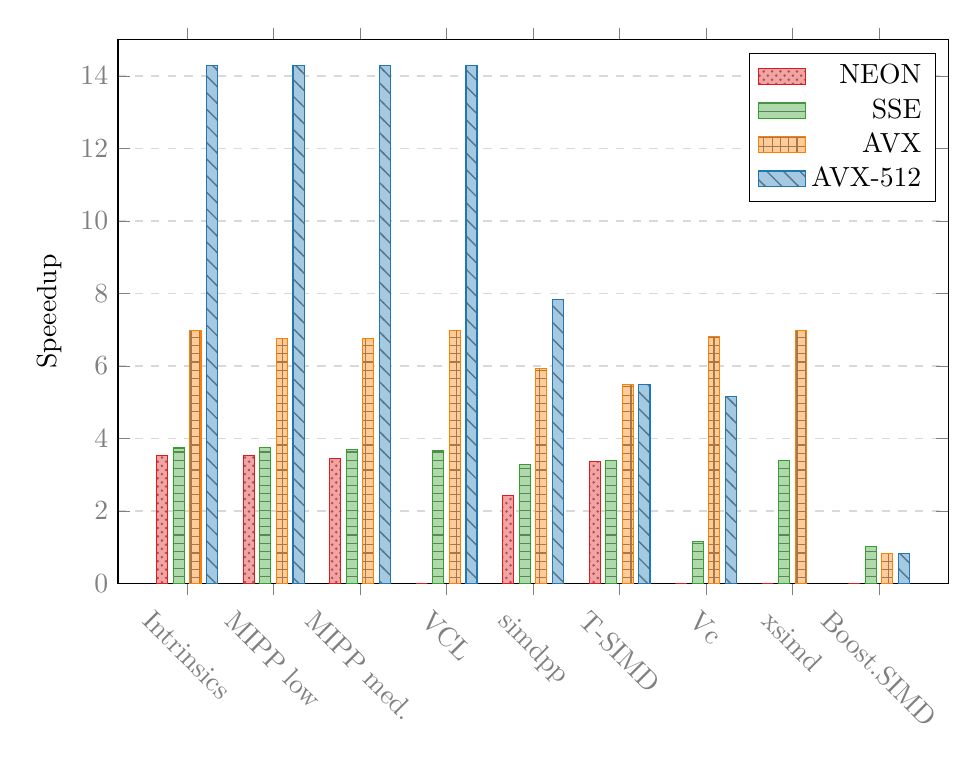
\begin{tikzpicture}
\begin{axis}[ybar,
             width=1.0\linewidth, height=0.700\linewidth,
             bar width=4pt,
             legend style={at={(0.985,0.975)}, anchor=north east,legend columns=1},
             legend cell align=right,
             area legend,
             ylabel={Speeedup}, ytick={0,2,...,14},
             symbolic x coords={intr,mippl,mippm,vcl,simdpp,tsimd,vc,xsimd,boost},
             xticklabel style={align=center, gray},
             yticklabel style={gray},
             xticklabels={Intrinsics,
                          MIPP low,
                          MIPP med.,
                          VCL,
                          simdpp,
                          T-SIMD,
                          Vc,
                          xsimd,
                          Boost.SIMD},
             xtick=data,
             ymajorgrids,
             grid style={dashed, gray!30},
             ymin=0,
             ymax=15,
             %nodes near coords,
             %nodes near coords align={vertical},
             every node near coord/.append style={rotate=90, anchor=west},
             x tick label style={rotate=-45},
             %label style={font=\large},
             %tick label style={font=\large},
             % tick align=outside, tickpos=left,
            ]

    % NEON
    \addplot[black!25!Paired-5,fill=Paired-5!40,draw=Paired-5,
             postaction={pattern color = black!50!Paired-5!70,
                         pattern=crosshatch dots}
            ]
            coordinates {(intr,3.52) (mippl,3.52) (mippm,3.45) (vcl,0) (simdpp,2.44) (tsimd,3.37) (vc,0) (xsimd,0) (boost,0)};
    \label{plot1}

    % SSE
    \addplot[black!25!Paired-3,fill=Paired-3!40,draw=Paired-3,
              postaction={pattern color = black!50!Paired-3!70,
                          pattern=horizontal lines}
             ]
             coordinates {(intr,3.74) (mippl,3.75) (mippm,3.70) (vcl,3.67) (simdpp,3.28) (tsimd,3.39) (vc,1.17) (xsimd,3.40) (boost,1.03)};
    \label{plot2}

    % AVX
    \addplot[black!25!Paired-7,fill=Paired-7!40,draw=Paired-7,
             postaction={pattern color = black!50!Paired-7!70,
                         pattern=grid}
            ]
            coordinates {(intr,6.98) (mippl,6.76) (mippm,6.76) (vcl,6.98) (simdpp,5.92) (tsimd,5.48) (vc,6.81) (xsimd,6.99) (boost,0.83)};
    \label{plot4}

    % AVX-512
    \addplot[black!25!Paired-1,fill=Paired-1!40,draw=Paired-1,
             postaction={pattern color = black!50!Paired-1!70,
                         pattern=flexible hatch north west}
            ]
            coordinates {(intr,14.30) (mippl,14.30) (mippm,14.30) (vcl,14.30) (simdpp,7.84) (tsimd,5.49) (vc,5.16) (boost,0.84)};
    \label{plot5}

    \legend{NEON,
            SSE,
            AVX,
            AVX-512,}
\end{axis}
\end{tikzpicture}
\end{document}
